\documentclass{article}
\usepackage[english,russian]{babel}
\usepackage{textcomp}
\usepackage{geometry}
  \geometry{left=2cm}
  \geometry{right=1.5cm}
  \geometry{top=1.5cm}
  \geometry{bottom=2cm}
\usepackage{tikz}
\usepackage{multicol}
\usepackage{listings}
\pagenumbering{gobble}

\lstdefinestyle{csMiptCppStyle}{
  language=C++,
  basicstyle=\linespread{1.1}\ttfamily,
  columns=fixed,
  fontadjust=true,
  basewidth=0.5em,
  keywordstyle=\color{blue}\bfseries,
  commentstyle=\color{gray},
  texcl=true,
  stringstyle=\ttfamily\color{orange!50!black},
  showstringspaces=false,
  numbersep=5pt,
  numberstyle=\tiny\color{black},
  numberfirstline=true,
  stepnumber=1,      
  numbersep=10pt,
  backgroundcolor=\color{white},
  showstringspaces=false,
  captionpos=b,
  breaklines=true
  breakatwhitespace=true,
  xleftmargin=.2in,
  extendedchars=\true,
  keepspaces = true,
  tabsize=4,
  upquote=true,
}
\lstdefinestyle{csMiptCppBorderStyle}{
  style=csMiptCppStyle,
  framexleftmargin=5mm, 
  frame=shadowbox, 
  rulesepcolor=\color{gray}
}

\lstset{style=csMiptCppStyle}
\lstset{literate={~}{{\raisebox{0.5ex}{\texttildelow}}}{1}}


\begin{document}
\title{Семинар \#1: Основы C++ \\[1ex] \large Пространства имён, ссылки, перегрузка функций, \texttt{std::string} и \texttt{std::vector}. \vspace{-5ex}}\date{}\maketitle



Язык C++ создан на основе языка C и одним из приоритетов языка является обратная совместимость с C. Поэтому почти любая программа на языке C будет работать и на языке C++.
Однако, нужно помнить, что это разные языки. В C++ было добавлено огромное количество новых возможностей, что сделало этот язык, вероятно, языком с самым большим количеством возможностей.

Для файлов исходного кода на языке C++ будем использовать расширение \texttt{.cpp}, а для заголовочных файлов расширение \texttt{.hpp}. Для компиляции программ на C++ будем использовать компилятор \texttt{g++}:
\begin{verbatim}
    g++ main.cpp
\end{verbatim}
Все библиотеки языка C доступны и в C++. Но для каждой библиотеки языка C в языке C++ есть своя (немного изменённая) версия этой библиотеки. Подключить эти библиотеки можно, используя те же названия, что и при подключении этих библиотек в C.
Но лучше использовать новые имена для этих библиотек, чтобы подчеркнуть, что это именно новая версия библиотеки из языка C. Для библиотеки \texttt{stdio.h} этим новым именем является \texttt{cstdio}. Для библиотеки \texttt{math.h} -- \texttt{cmath}, для \texttt{stdlib.h} -- \texttt{cstdlib} и так далее.
\begin{lstlisting}
#include <cstdio>
int main() 
{
    printf("Hello World\n");
}
\end{lstlisting}
Нужно отметить, что работа директивы \texttt{\#include} не отличается в языках C и C++. А \texttt{cstdio} является просто текстовым файлом (без расширения), лежащим в системной папке на диске.


\section*{Пространство имён (англ. \textit{namespace})}
Можем создавать пространство имён и писать внутри него код. Все объявленные внутри пространства имён сушности (например, переменные, функции, структуры) не видны напрямую вне пространства имён. Обратиться к ним можно по другому имени, состоящему из названия пространства имён, двух двоеточий и имени сущности:
\begin{lstlisting}
#include <cstdio>
namespace mipt 
{
    int a = 10;
    int square(int x)
    {
        return x * x;
    }
    struct point
    {
        int x, y;
    };
}

int main() 
{
    mipt::point p = {20, 30};
    printf("%i\n", mipt::square(mipt::a + p.x));
}
\end{lstlisting}
Кстати, обратите внимание, что в языке C++, в отличии от C, перед именем типа структуры не обязательно писать слово \texttt{struct}:
\begin{lstlisting}
struct point
{
    int x, y;
};

int main() 
{
    struct point p1;  // В C нужно было обязательно писать слово struct 
    point p2;         // В C++ можно не писать
}
\end{lstlisting}


\subsection*{Зачем нужны пространства имён?}
Представьте, что вы создаёте большую программу, исходный код который содержит миллионы строк кода. Конечно, большая часть кода написана не вами, так как вы используете библиотеки, написанные другими программистами.
Библиотекой можно назвать совокупность файлов исходного кода, нацеленных на решение какой-либо задачи. Например, есть библиотека для работы с графикой в которой содержатся функции/структуры/классы для работы с графикой. Или библиотека для работы с аудио, которая содежит функции/структуры/классы для обработки звука.

Если вы подключаете несколько библиотек, то существует высокая вероятность, что название чего-либо из одной библиотеки совпадёт с названием чего-то из другой библиотеки. Произойдёт так называемый конфликт имён. Конфликт имён, конечно, является ошибкой. Чтобы этого избежать и используются пространства имён.
\begin{lstlisting}
#include <cstdio>

namespace audio 
{
    int a = 10;
    int calculate(int x)
    {
        return x + 1;
    }
}

namespace graphics 
{
    int a = 20;
    int calculate(int x)
    {
        return x * 2;
    }
}

int main() 
{
    printf("%i\n", audio::a);     // 10
    printf("%i\n", graphics::a);  // 20
    printf("%i\n", graphics::calculate(audio::calculate(graphics::a)));  // 42
}
\end{lstlisting}

\subsection*{Директива \texttt{using namespace}}
Если вам очень не хочется постоянно писать названия пространства имён, то вы можете использовать директиву \texttt{using namespace}, которые добавляет все имена из некоторого пространства имён в текущее пространство имён:
\begin{lstlisting}
#include <cstdio>

namespace mipt 
{
    int a = 10;
    int square(int x)
    {
        return x * x;
    }
}

using namespace mipt;  // После этой строки mipt:: писать больше не нужно

int main() 
{
    printf("%i\n", square(a));
}
\end{lstlisting}
Использование такой возможности, конечно, полностью уничтожает всю пользу, которую приносят пространства имён. Поэтому, \texttt{using namespace} в своих программах лучше не использовать.

\subsection*{\texttt{using}-объявления}
Как правило пространство имён содержит огромное количество различных сущностей. Использование \texttt{using namespace} сделает видимыми сразу все имена из пространства имён и сильно увеличит вероятность возникновения конфликта имён. Но есть возможно сделать видимыми не все имена, а только несколько имён, используя ключевое слово \texttt{using} (без слова \texttt{namespace}): 
\begin{lstlisting}
#include <cstdio>

namespace mipt 
{
    int a = 10;
    int b = 20;
    int square(int x)
    {
        return x * x;
    }
}

using mipt::square, mipt::a; // После этой строки mipt:: не нужно писать для a и square

int main() 
{
    printf("%i\n", square(a + mipt::b));
}
\end{lstlisting}
Ключевое слово \texttt{using} можно использовать как вне всех функций, глобально, так и локально, внутри функций.

\newpage
\subsection*{Пространство имён \texttt{std}}
Все переменные/функции/структуры/классы стандартной библиотеки языка C++ содержатся в пространстве имён \texttt{std}. 


\subsection*{Печать на экран с помощью \texttt{std::cout}}
Рассмотрим глобальную переменную \texttt{cout} (сокращение от \textit{\textbf{c}haracter \textbf{out}put}), определённую в библиотеке \texttt{iostream} в пространстве имён \texttt{std}. Эта переменная и оператор \texttt{<{}<} используется для печати значения какого-либо объекта на экран:
\begin{verbatim}
    std::cout << объект;
\end{verbatim}
В результате этой операции объект напечатается на экран (если он может напечататься).
Результатом этой операции является всё тот же \texttt{std::cout}, поэтому можно применять \texttt{<{}<} несколько раз:
\begin{verbatim}
    std::cout << объект1 << объект2 << объект3;
\end{verbatim}
Использование \texttt{cout} и оператора \texttt{<{}<} является самым распространённым способом вывода текста на экран в C++.
\begin{lstlisting}
#include <iostream>
int main() 
{
    std::cout << "Hello, " << 123 << "\n";
}
\end{lstlisting}
В библиотеке \texttt{iostream} также есть такой объект, как \texttt{std::endl}. Если передать его объекту \texttt{cout} через оператор \texttt{<{}<} то напечатается перенос строки:
\begin{lstlisting}
#include <iostream>
int main() 
{
    std::cout << "Hello, " << 123 << std::endl;
}
\end{lstlisting}
Нужно отметить, что использование \texttt{std::endl} работает медленней, чем \texttt{\textbackslash n}, при печати в файл, так как вывод \texttt{std::endl} помимо печати переноса строки также сбрасывает всё содержимое буфера в файл.

\subsection*{Преемущество вывода \texttt{std::cout} перед \texttt{printf}}
Большим преемуществом использования \texttt{std::cout} перед функцией \texttt{printf} является то, что для \texttt{std::cout} не нужно указывать спецификатор типа, компилятор сам распознает тип передаваемого выражения.
\begin{lstlisting}
#include <iostream>
int main() 
{
    int a = 10;
    float b = 1.5;
    char c = 'A';
    
    std::cout << a << " " << b << " " << c << std::endl; // Напечатает 10 1.5 A
}
\end{lstlisting}

При этом, переменные типа \texttt{char} будут всегда печататься как символы. Если нужно напечатать переменную типа \texttt{char} как число, то нужно просто привести её тип к другому целочисленному типу:
\begin{lstlisting}
#include <iostream>
int main() 
{
    char c = 65;
    std::cout << c << " " << (int)c << std::endl;  // Напечатает  A 65
}
\end{lstlisting}


\subsection*{Считывание с экрана с помощью \texttt{std::cin}}
Глобальная переменная \texttt{cin} (сокращение от \textit{\textbf{c}haracter \textbf{in}put}), определённая в библиотеке \texttt{iostream} в пространстве имён \texttt{std} используется для считывания с экрана. Пример использования \texttt{std::cin}:
\begin{lstlisting}
#include <iostream>
int main() 
{
    int a, b;
    std::cin >> a >> b;               // Считали a и b
    std::cout << a + b << std::endl;  // Напечатали их сумму
}
\end{lstlisting}
\subsection*{Корректное использование функций из языка C в языке C++}
Вся стандартаная библиотека языка C++ лежит в пространстве имён \texttt{std}, поэтому любое имя из стандартной библиотеки начинается с \texttt{std::}. Это очень удобно, так как позволяет сразу увидеть в коде программы, какая сущность является стандартной, а какая нет. Однако, это не относится к сущностям пришедшим из языка C. Так как из-за обратной совместимости (C++ должен уметь компилировать программы на языке C) эти сущности должны работать без указания пространства имён \texttt{std}. Тем не меннее, даже для стандартных сущностей пришедших из языка C можно и нужно указывать пространство имён \texttt{std}.\\

\begin{minipage}{0.45\textwidth}
\quad \quad Некорректно
\begin{lstlisting}
#include <stdio.h>
#include <math.h>

int main() 
{
    printf("%f\n", sqrt(3));
}
\end{lstlisting}
\end{minipage}
\begin{minipage}{0.45\textwidth}
\quad \quad Корректно
\begin{lstlisting}
#include <cstdio>
#include <cmath>

int main() 
{
    std::printf("%f", std::sqrt(3));
}
\end{lstlisting}
\end{minipage}


\subsection*{Пространства имён и отступы}
Внутри пространств имён НЕ следует делать дополнительный отступ. Использование отступа внутри пространства имён является примером плохого стиля кода. В примерах этой главы отступ делался, чтобы код был более понятным. В реальности код пространства имён должен выглядеть как-то так:
\begin{lstlisting}
#include <iostream>
namespace mipt 
{
int a = 10;
int square(int x)
{
    return x * x;
}
struct point
{
    int x, y;
};
}

int main()
{
    std::cout << mipt::square(5) << std::endl;
}
\end{lstlisting}
\newpage
\section*{Ссылки}
В C++ вводится понятие нового типа под названием ссылка.
Ссылку можно представить себе как такой необычный указатель, который всегда указывает в одно место и который сам автоматически разыменовывается при использовании. Ссылки заменяют указатели в некоторых ситуациях, так как ими удобнее пользоваться.

Тип ссылки состоит из названия типа, на который указывает ссылка + значок амперсанда (\texttt{\&}). Например, ссылка на \texttt{int} будет иметь тип \texttt{int\&}.

Пусть есть переменная \texttt{a}. Давайте создадим указатель и ссылку на эту переменную и увеличим её на 1 с помощью указателя/ссылки:
\begin{multicols}{2}
Используем указатель
\begin{lstlisting}
int a = 10;
int* p = &a;
*p += 1;
\end{lstlisting}

Используем ссылку
\begin{lstlisting}
int a = 10;
int& r = a;
r += 1;
\end{lstlisting}
\end{multicols}

\textbf{\large{!}} \quad Не стоит путать \texttt{\&} используемый при объявлении ссылки и \texttt{\&} используемый для нахождения адреса переменной. Это разные \texttt{\&}, никак друг с другом не связанные.\\

Ссылками удобно пользоваться потому что:
\begin{enumerate}
\item При создании ссылки нам не нужно передавать ей адрес. Просто передаём ей некоторый объект, а ссылка уже сама находит его адрес.
\item Ссылку не нужно разыменовывать, она разыменовывается сама.
\end{enumerate}
При работе ссылками важно помнить, что все (почти) операции применяемые к ссылке, на самом деле применяются  к объекту на который эта ссылка указывает. Это происходит потому что ссылка (почти) всегда сама разыменуется.
\begin{lstlisting}
#include <iostream>
using std::cout, std::endl;
int main() 
{
    int a = 10;
    int& r = a;

    r += 5;                     // Прибавим к a число 5
    r *= 2;                     // Умножим a на 2
    cout << r << endl;          // Напечатаем a
    cout << sizeof(r) << endl;  // Напечатаем размер a
    cout << &r << endl;         // Напечатаем адрес a
}
\end{lstlisting}
Также, как и указатели, ссылки могут указывать не только на переменные, но и на другие объекты, такие как элементы массива или структуры.
\begin{lstlisting}
#include <iostream>
int main() 
{
    int a[5] = {10, 20, 30, 40, 50};

    int& r = a[1];
    r += 1;

    std::cout << a[1] << std::endl;  // Напечатает 21
}
\end{lstlisting}

\newpage
\subsection*{Отличия ссылок и указателей}
Несмотря на то, что ссылки и указатели во многом похожи, у них есть и много существенных отличий.
\begin{enumerate}
\item \textbf{Указатель можно создать без инициализации, а ссылку обязательно нужно инициализировать}

То есть, указатель можно создать так:
\begin{lstlisting}
int* p;
\end{lstlisting}
В этом случае в \texttt{p} будет храниться произвольный адрес. Разыменовывать такой указатель, не задав его значение адресом какого-либо объекта, очень опасно -- это приведёт к неопределённому поведению.

Ссылку же нельзя создать без инициализации, то есть такая строка будет ошибкой:
\begin{lstlisting}
int& r;  // Ошибка компиляции
\end{lstlisting}
При создании ссылки нужно обязательно указать то, на что она будет указывать


\item \textbf{Указатель может быть нулевым, а ссылка нет}

Указатель можно приравнять нулевому значению, равному \texttt{NULL} или \texttt{nullptr}. Разыменование такого нулевого указателя приведёт к ошибке.

Ссылку же нельзя инициализировать никаким нулевым значением.
То есть не существует никакой константы, которая бы обозначала нулевую ссылку.

\item\textbf{ Указатель можно переприсвоить, а ссылку нет}

Если указатель \texttt{p} сначала указывал в одно место, например, на переменную \texttt{a}, то можно просто написать:
\begin{lstlisting}
p = &b;
\end{lstlisting}
и указатель станет указывать на переменную \texttt{b}.

Со ссылками такое не пройдёт, они всегда указывают на тот объект, который был указан при создании ссылки.
При попытке изменить это и написать что-то вроде:
\begin{lstlisting}
r = b;
\end{lstlisting}
ссылка автоматически разыменуется и присваивание произойдёт к тому, на что указывает ссылка.

\item \textbf{У указателей есть арифметика указателей, а у ссылок нет}

К указателю можно прибавлять/отнимать целые числа. Можно вычесть 2 указателя. Можно применить \texttt{[]} к указателю.

Ничего такого со ссылками сделать нельзя. При попытке прибавить к ссылке число, оно прибавится к той 
переменной, на которую указывает ссылка, так как ссылка автоматически разыменуется.

\item \textbf{Ссылки это не совсем обычный объект, некоторые операции с ними запрещены}

Нельзя создать массив из ссылок. Нельзя получить адрес ссылки (если применим \texttt{\&} к ссылке то вернётся адрес того объекта на который указывет ссылка). Нельзя создать указатель на ссылку. Нельзя создать ссылку на ссылку.
\begin{lstlisting}
int x = 1, y = 2, z = 3;

int* a[3] = {&x, &y, &z};  // ОК, массив из указателей
int& b[3] = {x, y, z};     // Ошибка, создать массив из ссылок нельзя


int* p = &x;
int** q = &p;  // ОК, указатель на указатель

int& r = x;
int&& s = r;  // Ошибка, нельзя создать ссылку на ссылку
int& t = r;   // ОК, ссылка r сама разыменуется и t будет указывать на x 
\end{lstlisting}
\end{enumerate}

\newpage

\subsection*{Константные ссылки}
Используя константную ссылку нельзя изменить объект на который она указывает:
\begin{lstlisting}
int a = 10;
const int& r = a;
r += 1;             // Ошибка, нельзя изменить a, так как ссылка константная
\end{lstlisting}
Константные ссылки могут привязываться как к константам, так и не константам:
\begin{lstlisting}
int a = 10;
const int b = 20;
    
int& r1 = a;        // OK
int& r2 = b;        // Ошибка, нельзя привязать обычную ссылку к константе

const int& c1 = a;  // OK
const int& c2 = b;  // OK
\end{lstlisting}
Удивительной особеностью константных ссылок является то, что они могут привязываться не только к объектам, лежащим в памяти, но и к "временным"{} объектам у которых нет адреса:
\begin{lstlisting}
int a = 10;
    
int& r1 = a + 1;        // Ошибка, выражению a + 1 не соответствует никакой объект в памяти
int& r2 = 20;           // Ошибка, выражению 20 не соответствует никакой объект в памяти

const int& c1 = a + 1;  // OK
const int& c2 = 20;     // OK
\end{lstlisting}
После этого можно корректно пользоваться ссылками \texttt{c1} и \texttt{c2}, их значения будут равны \texttt{11} и \texttt{20}.

\subsection*{Передача по ссылке в функции}
Чаще всего ссылки используются для того чтобы передать что либо в функцию. Часто нам хочется передать переменную в функцию и изменить её внутри функции. Это можно делать и с помощью указателей, но с помощью ссылок это делать гораздо удобней. Рассмотрим две программы:

\begin{multicols}{2}
Передаём по указателю:
\begin{lstlisting}
#include <iostream>
void square(int* p)
{
    *p = *p * *p;
}

int main()
{
    int a = 5;
    square(&a);
    std::cout << a << std::endl;
}
\end{lstlisting}

Передаём по ссылке:
\begin{lstlisting}
#include <iostream>
void square(int& a)
{
    a = a * a;
}

int main()
{
    int a = 5;
    square(a);
    std::cout << a << std::endl;
}
\end{lstlisting}
\end{multicols}

Обратите внимание на 2 вещи:
\begin{enumerate}
\item Ссылку не нужно разыменовывать внутри функции, это происходит автоматически.
\item При передаче в функцию, не нужно передавать адрес переменной. Нужно передать саму переменную, её адрес вычислится автоматически. При этом копирования объекта в функцию не происходит, ссылки работают также быстро как и указатели.
\end{enumerate}


\subsection*{Передача по константной ссылке в функции}
Даже если мы не хотим менять объект внутри функции, мы всё-равно можем захотеть передать его по ссылке, так как передача по ссылке не копирует объект, следовательно гораздо более эффективна для больших объектов, чем передача по значению. В этом случае очень важно передавать объект именно по константной ссылке, так как это будет явно показывать, что объект не изменится внутри функции.
\begin{lstlisting}
#include <iostream>
struct Book
{
    char title[100];
    int pages;
    float price;
};

void printTitleValue(Book b)
{
    std::cout << b.title << std::endl;
}

void printTitleRef(Book& b)
{
    std::cout << b.title << std::endl;
}

void printTitleCRef(const Book& b)
{
    std::cout << b.title << std::endl;
}

int main() 
{
    Book b = {"Harry Potter", 100, 200};

    printTitleValue(b);  // Медленно, так как структура будет копироваться
    
    printTitleRef(b);    // Быстро, но мы не можем быть уверены, что структура 
                         // не изменится в функции
                         
    printTitleCRef(b);   // Самый лучший способ в этом случае
}
\end{lstlisting}


\subsection*{Три способа передачи объекта в функцию в языке C++}

\begin{enumerate}
\item Передача по значению: \quad \texttt{void func(Object a)}

Используйте этот способ если объект маленький и вы не хотите изменять его внутри функции.

\item Передача по ссылке: \quad \texttt{void func(Object\& a)}

Используйте этот способ если вы хотите изменить объект внутри функции.

\item Передача по константной ссылке: \quad \texttt{void func(const Object\& a)}

Используйте этот способ если объект большой и вы не хотите изменять его внутри функции.
\end{enumerate}



\subsection*{Возврат ссылок из функций}
Ссылки можно и возвращать из функции. Например, в данном примере, функция \texttt{get} возвращает ссылку на глобальную переменную \texttt{x}:
\begin{lstlisting}
#include <iostream>
int x = 10;

int& get() 
{
    return x;
}

int main() 
{
    get() = 20;
    std::cout << x << std::endl;      //  Напечатает 20
}
\end{lstlisting}
Необычное свойство функций, которые возвращают ссылки, заключается в том, что выражение вызова функции может стоять слева от знака присваивания.\\

Как это работает:
\begin{itemize}
\item Функция \texttt{get} возвращает ссылку на глобальную переменную \texttt{x}. То есть за место \texttt{get()} подставится ссылка на \texttt{x}.

\item Так как ссылки автоматически разыменуются и так как ссылка, возвращённая из функции, указывает на \texttt{x}, то на место \texttt{get()} по сути подставится сам \texttt{x}. 
\end{itemize}

\subsection*{Возврат ссылок на локальные переменные. Висячие ссылки.}
При возврате ссылки из функции нужно следить за тем, чтобы функция не вернула ссылку на локальную переменную, как это происходит в данном примере. После завершения функции \texttt{get}, переменная \texttt{x} удалится, так как она была определена внутри функции. В результате, внутри функции \texttt{main} мы попробуем доступиться к области памяти, в которой раньше лежала переменная \texttt{x}. Это приведёт к неопределённому поведению.
\begin{lstlisting}
#include <iostream>

int& get() 
{
    int x = 10;
    int& r = x;
    return r;
}

int main() 
{
    int& r = get();
    r += 1;  // Пытаемся изменить переменную x, которая уже удалена, это UB
}
\end{lstlisting}

Ссылки, которые указывают на уже удалённый объект в памяти называются висячими ссылками (англ. \textit{dangling references}).

\newpage
\subsection*{Функции, которые принимают ссылку и возвращают её же}
Интересный и часто встречающийся случай -- это когда функция принимает ссылку, а потом возвращает её же. Например, в данном примере, функция \texttt{inc} принимает ссылку, увеличивет то, на что указывает эта ссылка на \texttt{1}, а затем возвращает эту ссылку. При этом никакого копирование самой переменной \texttt{a} в функцию и из функции не происходит.

Также это безопасно, ведь теперь возвращаемая ссылка будет указывать не на локальную переменную функции \texttt{inc}, а туда же, куда указывала ссылка \texttt{r}, пришедшая на вход функции. И при завершении функции \texttt{inc}, объект, на который указывает возвращаемая ссылка (переменная \texttt{a}), не удалится.
\begin{lstlisting}
#include <iostream>
int& inc(int& r) 
{
    r += 1;
    return r;
}
int main() 
{
    int a = 10;
    inc(a);
    std::cout << a << std::endl;  // Напечатает 11
    
    inc(a) += 5;
    std::cout << a << std::endl;  // Напечатает 17
    
    inc(inc(inc(a)));
    std::cout << a << std::endl;  // Напечатает 20
}
\end{lstlisting}


\section*{Перегрузка функций}

Пусть у нас есть задача -- нужно написать функцию, которая бы вычисляла модуль числа. Такую функцию несложно написать, но только с числами какого типа будет работать эта функция? Ведь если мы напишем такую функцию для чисел типа \texttt{int}, она не будет работать с числами типа \texttt{double}. По хорошему, придётся писать такую функцию для каждого числового типа, чтобы мы могли бы находить модуль любого числа. 

В языке C придётся писать функции для каждого типа и давать каждой функции уникальное имя:
\begin{lstlisting}
#include <stdio.h>
int abs(int a)
{
    if (a < 0)
        return -a;
    return a;
}
double fabs(double a)
{
    if (a < 0)
        return -a;
    return a;
}
int main()
{
    double x = abs(-1.5);   // Ошиблись - используем не ту функцию!
    printf("%lf\n", x);     // Напечатает 1.0
}
\end{lstlisting}
Такой подход имеет следующие проблемы:

\begin{enumerate}
\item Придётся придумывать и запоминать разные странные названия функций для разных входных типов. Например, в стандартной библиотеке языка C для нахождения модуля чисел типа \texttt{float} используется функция \texttt{fabsf}, а для чисел типа \texttt{long long} -- функция \texttt{llabs}.

\item Легко случайно ошибиться и вызвать функцию для другого типа. Потом такую ошибку может быть непросто обнаружить.

\item Приходится писать много похожих функций. Грубо говоря, каждую функцию придётся повторить несколько раз - по одному разу для каждого числового типа. Получается очень много кода.
\end{enumerate}
В языке C++ добавлена возможность, которая поможет нам решить первые две проблемы. Эта новая возможность языка называется \textit{перегрузка функций} и она позволяет нам писать разные функции с одинаковыми именами, если у этих функций различаются типы параметров и/или их количество. Функции, которые используют механизм перегрузки функций, называются перегруженными функциями или просто перегрузками.

Теперь, если мы будем использовать С++ и перегрузку функций,  пример выше перепишется так:
\begin{lstlisting}
#include <iostream>
int abs(int a)
{
    if (a < 0)
        return -a;
    return a;
}

double abs(double a)
{
    if (a < 0)
        return -a;
    return a;
}

int main()
{
    double x = abs(-1.5);         // Всё правильно, abs можно передавать и int и double
                                  // компилятор сам выберет нужную перегрузку
    std::cout << x << std::endl;  // Напечатает 1.5
}
\end{lstlisting}


\subsection*{Как можно перегружать функции}

\begin{itemize}
\item Функции можно перегружать по типу аргументов:
\begin{lstlisting}
#include <iostream>

void func(int a)    {std::cout << "Int"    << std::endl;}
void func(double a) {std::cout << "Double" << std::endl;}

int main()
{
    func(1);    // Напечатает Int
    func(1.5);  // Напечатает Double
}
\end{lstlisting}

\newpage
\item Функции можно перегружать по количеству аргументов:
\begin{lstlisting}
#include <iostream>

void func()             {std::cout << "Zero" << std::endl;}
void func(int a)        {std::cout << "One"  << std::endl;}
void func(int a, int b) {std::cout << "Two"  << std::endl;}

int main()
{
    func();        // Напечатает Zero
    func(10);      // Напечатает One
    func(10, 20);  // Напечатает Two
}
\end{lstlisting}

\item Можно перегрузить по обычной ссылке и константной ссылке:
\begin{lstlisting}
#include <iostream>

void func(int& a)        {std::cout << "Ref"  << std::endl;}
void func(const int& a)  {std::cout << "CRef" << std::endl;}

int main()
{
    int a = 10;
    const int b = 20;
    
    func(a);       // Напечатает Ref
    func(b);       // Напечатает CRef
    
    func(30);      // Напечатает CRef
    func(a + 1);   // Напечатает CRef
}
\end{lstlisting}
\end{itemize}

\subsection*{Как нельзя перегружать функции}

\begin{itemize}
\item Функции нельзя перегружать по типу возвращаемого значения:
\begin{lstlisting}
#include <iostream>

int func(int a)     {std::cout << "Int"    << std::endl;}
double func(int a)  {std::cout << "Double" << std::endl;}

int main()
{
    func(1);  // Невозможно выбрать
}
\end{lstlisting}
\end{itemize}


\newpage
\subsection*{Неодназначности при выборе перегрузки}
Так как в языке C++ также есть такая вещь, как неявное приведение типов, то может так оказаться, что в качестве перегрузки подойдут несколько функций. Какая из функций будет при этом выбираться? Рассмотрим это на нескольких примерах:

\begin{itemize}
\item Известно, что числа типа \texttt{float} можно присваивать числам типа \texttt{double} и наоборот. При этом происходит неявное приведение типов. Соответственно, числа типа \texttt{float} также можно передавать в функции, которые принимают \texttt{double}. Но что если есть две перегрузки, одна принимает \texttt{float}, а другая -- \texttt{double} и мы передаём число типа \texttt{float}. Оба варианта подходят. Какая из перегрузок выберется?
\begin{lstlisting}
#include <iostream>

void func(float a)  {std::cout << "Float"  << std::endl;}
void func(double a) {std::cout << "Double" << std::endl;}

int main()
{
    float x = 1.5f;
    func(x);  // Напечатает Float
}
\end{lstlisting}
В этом случае выберется перегрузка с \texttt{float}, так как она лучше подходит.

\item Что если у нас есть две перегрузки: одна с \texttt{int}, а другая с \texttt{double}, а мы передаём в функию число \texttt{float}. Опять обе функции подходят. Какая из перегрузок выберется на этот раз?
\begin{lstlisting}
#include <iostream>

void func(int a)    {std::cout << "Int"    << std::endl;}
void func(double a) {std::cout << "Double" << std::endl;}

int main()
{
    float x = 1.5f;
    func(x);  // Напечатает Double
}
\end{lstlisting}
В этом случае выберется перегрузка с \texttt{double}. Она лучше подходит, так как при преобразовании \texttt{float} в \texttt{double} не происходит потери точности числа, а при преобразовании \texttt{float} в \texttt{int} такая потеря точности может произойти. Поэтому тут выбирается перегрузка с \texttt{double}.

\item Что если у нас есть две перегрузки: одна с \texttt{int}, а другая с \texttt{float}, а мы передаём в функцию число \texttt{double}. Опять обе функции подходят. Но в обоих вариантах будет происходить потеря точности. Какая из перегрузок выберется на этот раз?
\begin{lstlisting}
#include <iostream>

void func(int a)   {std::cout << "Int"   << std::endl;}
void func(float a) {std::cout << "Float" << std::endl;}

int main()
{
    double x = 1.5;
    func(x);  // Ошибка компиляции
}
\end{lstlisting}
В этот раз компилятор не сможет выбрать правильную перегрузку, так как в этом случае обе функции подходят одинаково хорошо. Интересно, что если в этом примере одну из функции просто удалить, то программа скомпилируется без ошибки.
\end{itemize}

\subsection*{Перегрузка на более сложных типах}
Перегрузка часто применяется к функциям принимающим объекты пользовательских типов, таких как структуры или классы.
\begin{lstlisting}
#include <iostream>

struct Book
{
    char title[100];
    int numPages;
};

struct Movie
{
    char title[100];
    float rating;
};

void printTitle(const Book& b)
{
    std::cout << b.title << std::endl;
}

void printTitle(const Movie& m)
{
    std::cout << m.title << std::endl;
}

int main()
{
    Book b = {"Harry Potter", 500};
    Movie m = {"The Matrix", 9.0};
    
    printTitle(b);  // Напечатает  Harry Potter
    printTitle(m);  // Напечатает  The Matrix
}
\end{lstlisting}


\newpage
\section*{Строка языка C++. Класс \texttt{std::string}.}

Как известно, строки в языке C являются просто массивами символов (элементов типа \texttt{char}). Использовать такие строки не очень удобно, так как нужно постоянно следить, чтобы строка вмещалась в массив в котором она хранится. При этом легко ошибиться и выйти за границы этого массива, что приведёт к неопределённому поведению. Также строки в языке C неудобно присваивать, конкатенировать и сравнивать -- для этих операций требуется использовать функции из библиотеки \texttt{string.h}.

В языке C++ появляется гораздо более удобный способ работы со строками -- использование класса \texttt{std::string} из библиотеки \texttt{string} (не путайте эту библиотеку с библиотекой \texttt{string.h}, также известной как \texttt{cstring}). Работая со строкам \texttt{std::string} можно не задумываться о выделении/освобождении памяти -- всё будет сделано автоматически. Также такие строки удобно присваивать, складывать и сравнивать.

При этом использовать старые строки из языка C тоже можно, в языке C++ такие строки называются \textit{C-строками}.
\begin{lstlisting}
#include <iostream>
#include <cstring>  // Библиотека для работы с C-строками. Содержит strlen, strcpy и т. д.
#include <string>   // Библиотека, содержащая класс std::string

int main()
{
    // Работаем с C-строками в языке C++
    char a[50] = "Cat";
    std::strcpy(a, "Mouse");
    std::strcat(a, "Dog");
    
    if (std::strcmp(a, "MouseDog") == 0)
        std::cout << a << std::endl;
        
        
    // Проделаем аналогичные операции, используя класс std::string
    std::string b = "Cat";
    b = "Mouse";
    b += "Dog";
    
    if (b == "MouseDog")
        std::cout << b << std::endl;
}
\end{lstlisting}

\subsection*{Манипуляция с отдельными символами в строках \texttt{std::string}}
Работа с отдельными символами в строках \texttt{std::string} происходит также, как и в C-строках.
Элемент строки \texttt{std::string} тоже является символом типа \texttt{char}. Выход за границы также является неопределённым поведением.
\begin{lstlisting}
#include <iostream>
#include <string>
int main()
{
    std::string a = "Mouse";
    std::cout << a[0] << std::endl;  // Напечатает M
    
    a[4] = 'X';
    std::cout << a << std::endl;     // Напечатает MousX
    
    a[10] = 'X'; // UB
}
\end{lstlisting}
Для работы с символами можно использовать библиотеку \texttt{ctype.h} из языка C, в C++ она называется \texttt{cctype}:
\begin{lstlisting}
#include <iostream>
#include <string>
#include <cctype>
int main()
{
    std::string s = "Mouse123!";
    for (std::size_t i = 0; i < s.size(); ++i)
    {
        if (std::isalpha(s[i]))
            s[i] += 1;
    }
    std::cout << s << std::endl;  // Напечатает Npvtf123!
}
\end{lstlisting}



\subsection*{Методы класса \texttt{std::string}}
\textit{Класс} -- это пользовательский тип данных, который позволяет объединять данные и функции, работающие с этими данными, в одну сущность.

\textit{Методы класса} -- это функции, определенные внутри класса, которые описывают поведение объектов этого класса. Вызов методов класса осуществляется на объектах класса с помощью оператора точка.

Рассмотрим методы класса \texttt{std::string}:
\begin{itemize}
\item Метод \texttt{push\_back} -- добавляет один символ в конец строки.
\item Метод \texttt{pop\_back} -- удаляет один символ из конца строки.
\begin{lstlisting}
#include <iostream>
#include <string>
int main()
{
    std::string s = "Elephant";
    s.push_back('X');
    std::cout << s << std::endl;  // Напечатает ElephantX
    
    s.pop_back();
    s.pop_back();
    std::cout << s << std::endl;  // Напечатает Elephan
}
\end{lstlisting}

\item Метод \texttt{insert} -- добавляет символы в строку.
\item Метод \texttt{clear} -- очищает строку.
\begin{lstlisting}
#include <iostream>
#include <string>
int main()
{
    std::string s = "Elephant";
    s.insert(2, "Cat");           // Начиная с символа с индексом 2, добавь Cat
    std::cout << s << std::endl;  // Напечатает ElCatephant
    
    s.clear();
    std::cout << s << std::endl;         // Напечатает пустую строку
    std::cout << s.size() << std::endl;  // Напечатает 0
}
\end{lstlisting}

\item Метод \texttt{erase} -- удаляет символы из строки.
\begin{lstlisting}
#include <iostream>
#include <string>
int main()
{
    std::string s = "Elephant";
    s.erase(2, 4);                // Начиная с символа с индексом 2, удали 4 символа
    std::cout << s << std::endl;  // Напечатает Elnt
}
\end{lstlisting}


\item Метод \texttt{substr} -- получает подстроку из строки. При этом создаёт новую строку и копирует туда часть изначальной строки.
\begin{lstlisting}
#include <iostream>
#include <string>
int main()
{
    std::string s = "Elephant";
    std::string a = s.substr(2, 4);  // Начиная с символа с индексом 2, 
                                     // возьми подстроку длины 4
    std::cout << a << std::endl;     // Напечатает epha
}
\end{lstlisting}


\item Метод \texttt{find} -- ищет подстроку в строке. Возвращает индекс первого символа первого вхождения подстроки (тип \texttt{std::size\_t}). В случае, если найти подстроку не удалось, возвращает числовую константу \texttt{std::string::npos}.
\begin{lstlisting}
#include <iostream>
#include <string>
using std::cout, std::endl, std::size_t;
int main()
{
    std::string s = "Elephant";
    size_t k = s.find("phan");
    
    if (k != std::string::npos)
        cout << "Found, index = " << k << endl;
    else
        cout << "Not found" << endl;
}
\end{lstlisting}
Данная программа напечатает \texttt{Found, index = 3}.

\item Метод \texttt{starts\_with} -- проверяет, начинается ли строка данного префикса. Метод \texttt{ends\_with} -- проверяет, кончается ли строка на данный суффикс. Методы возращают значение типа \texttt{bool}.
\begin{lstlisting}
#include <iostream>
#include <string>
int main()
{
    std::string s = "Elephant";
    
    if (s.starts_with("Ele"))
        std::cout << "Yes" << std::endl;
}
\end{lstlisting}


\end{itemize}

\subsection*{Внутреннее устройство объектов типа \texttt{std::string}}

Строки типа \texttt{std::string} представляют собой не что иное, как динамический массив из элементов типа \texttt{char}. Реализация строки может отличаться в стандартных библиотеках разных компиляторов, но в большинстве реализации строка имеет примерно следующее строение. В самом объекте строки хранятся указатель на данные, размер строки и её вместимость. Указатель хранит адрес на массив элементов типа \texttt{char}, который хранится в куче.\\
Рассмотрим строку:
\begin{lstlisting}
std::string a = "Cats and dogs and elepnants";
\end{lstlisting}
Её можно представить в памяти следующим образом:
\begin{center}
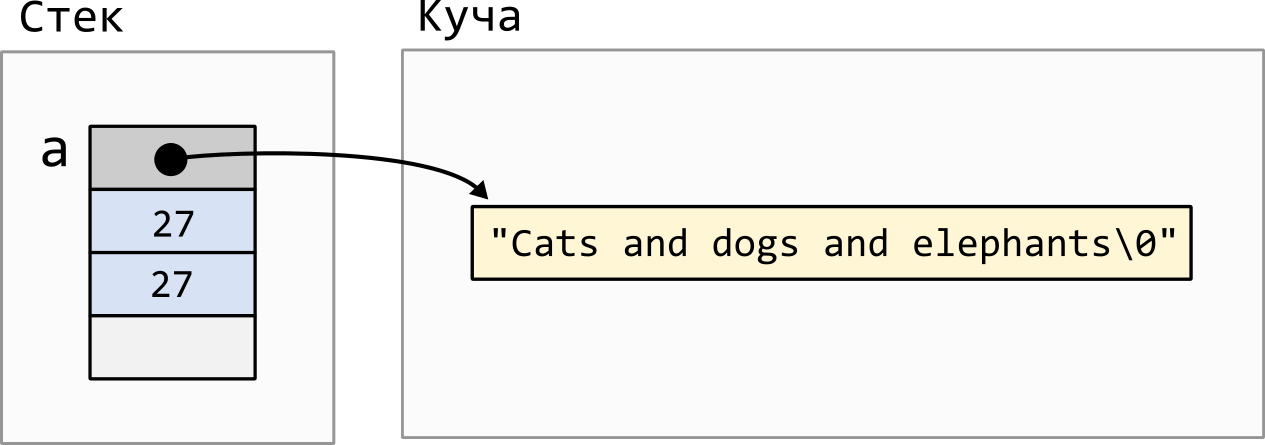
\includegraphics[scale=1]{../images/large_string.png}
\end{center}
Обратите внимание, на следующие моменты:

\begin{itemize}
\item Нулевой символ \texttt{\textbackslash 0} также хранится на конце строки, несмотря на то что размер строки мы храним и могли бы обойтись без нулевого символа. Это делается для того, чтобы можно было легко передавать содержимое \texttt{std::string} в функцию, которая принимает C-строку. В такую функцию достаточно будет передать указатель на данные в куче.
\item Размер и вместимость хранятся без учёта нулевого символа. То есть, если вместимость равна 27, то реально в куче выделяется 28 байт.
\item Размер самого объекта строки равен 32 байта, последние 8 байт могут быть не заняты. Эти 8 байт нужны, для так называемой \textit{оптимизации малой строки}. Об этой оптимизации будет рассказано в следующем семинаре.
\end{itemize}

\subsection*{Дополнительные методы класса \texttt{std::string}}

\begin{itemize}
\item Метод \texttt{c\_str()} -- возвращает указатель на данные в куче.
\item Метод \texttt{size()} -- возвращает размер строки.
\item Метод \texttt{capacity()} -- возвращает вместимость строки.
\item Метод \texttt{reserve(size\_t n)} -- увеличивает вместимость строки.
\item Метод \texttt{resize(size\_t n)} -- изменяет размер строки.
\item Метод \texttt{shrink\_to\_fit()} -- делает вместимость строки, равной её размеру.
\begin{lstlisting}
#include <iostream>
#include <string>
int main()
{
    std::string a = "Cats and dogs and elepnants";
    std::cout << a.size() << " " << a.capacity() << std::endl;  // Напечатает 27 27
    
    a += "!";
    std::cout << a.size() << " " << a.capacity() << std::endl;  // Напечатает 28 54
    
    a.shrink_to_fit();
    std::cout << a.size() << " " << a.capacity() << std::endl;  // Напечатает 28 28
}
\end{lstlisting}
\end{itemize}



\subsection*{Передача строк в функции}
При передаче строки в функцию по значению происходит глубокое копирование строки, что может быть медленно, если строка большая. Поэтому лучше строки передавать по ссылке. Следуют передавать строку по обычной ссылке, если вы хотите изменить строку внутри функции и передавать строку по константной ссылке, если не хотите изменять строку.
\begin{lstlisting}
#include <iostream>
#include <string>
#include <cctype>
using std::cout, std::endl, std::size_t;

// Переводим все буквы строки в верхний регистр. Передаём по ссылке.
void convertToUpper(std::string& s)
{
    for (size_t i = 0; i < s.size(); ++i)
    {
        s[i] = std::toupper(s[i]);
    }
}
// Считаем количество букв в строке. Обязательно нужно передавать по константной ссылке.
size_t countLetters(const std::string& s)
{
    size_t result = 0;
    for (size_t i = 0; i < s.size(); ++i)
    {
        if (std::isalpha(s[i]))
            result += 1;
    }
    return result;
}

// При передаче строки в эту функцию, строка будет копироваться, это плохо
void badFunction(std::string s)
{
    std::cout << s << std::endl;
}

int main()
{
    std::string a = "Mouse123Cat!";
    cout << a << endl;                // Напечатает Mouse123Cat!
    
    convertToUpper(a);
    cout << a << endl;                // Напечатает MOUSE123CAT!
    cout << countLetters(a) << endl;  // Напечатает 8
    
    badFunction(a);  // Произойдёт копирование строки a в функцию badFunction
}
\end{lstlisting}

\newpage

\subsection*{Передача строк \texttt{std::string} в функции языка C}
Метод \texttt{c\_str} класса \texttt{std::string} возвращает указатель на данные в куче. Этот метод можно использовать если нужно передать содержимое строки \texttt{std::string} в функцию, которая принимает C-строку.
\begin{lstlisting}
#include <iostream>
#include <cstring>
#include <string>

int main()
{
    std::string a = "Cat";
    
    char b[10];
    std::strcpy(b, a.c_str());

    std::cout << b << std::endl;  // Напечатает Cat
}
\end{lstlisting}


\subsection*{Конвертация чисел в строки и наоборот}
Для конвертации чисел в строки можно использовать функцию \texttt{std::to\_string}. Эта функция может принимать числа любых типов, так как тут используется механизм перегрузки функций.
\begin{lstlisting}
#include <iostream>
#include <string>

int main()
{
    int a = 123;
    std::string sa = std::to_string(a);
    std::cout << sa << std::endl;  // Напечатает 123
    
    float x = 123.456;
    std::string sx = std::to_string(x);
    std::cout << sx << std::endl;  // Напечатает 123.456
}
\end{lstlisting}
Для конвертации из строки в число следует использовать функции \texttt{std::stoi} (для чисел типа \texttt{int}), \texttt{std::stof} (для чисел типа \texttt{float}),  \texttt{std::stod} (для чисел типа \texttt{double}) и так далее. Тут нельзя было применить перегрузку функций, так как функции различаются только по возращаемому значению.
\begin{lstlisting}
#include <iostream>
#include <string>

int main()
{
    std::string sa = "123";
    int a = std::stoi(sa);
    std::cout << a << std::endl;  // Напечатает 123
    
    std::string sx = "123.456";
    float x = std::stof(sx);
    std::cout << x << std::endl;  // Напечатает 123.456
}
\end{lstlisting}


\subsection*{Передача C-строк в функции, которые принимают \texttt{std::string}}
Что, если мы передаём C-строку в функцию, которая принимает строку типа \texttt{std::string}? Кажется, это работать не должно, так как типы не совпадают. Но, на самом деле это работает автоматически, если функция принимает строку по значению или по константной ссылке. Рассмотрим это на примере:
\begin{lstlisting}
#include <iostream>
#include <string>
using std::cout, std::endl;

void func1(std::string str)        {cout << str << endl;}
void func2(std::string& str)       {cout << str << endl;}
void func3(const std::string& str) {cout << str << endl;}

int main()
{
    char a[10] = "Cat";
    func1(a);  // OK
    func2(a);  // Ошибка
    func3(a);  // OK
}
\end{lstlisting}



\subsection*{Литералы типа \texttt{std::string}}
Строковые литералы в языках C и C++ не отличаются. Это простые массивы элементов типа \texttt{char}, хранящиеся в сегменте данные. Строковые литералы имеют тип \texttt{const char[n]}, где \texttt{n} -- это размер строки включая \texttt{\textbackslash 0}. 
\begin{lstlisting}
#include <iostream>
#include <string>

void func(const char* str)        {std::cout << "C-string" << std::endl;}
void func(const std::string& str) {std::cout << "std::string" << std::endl;}

int main()
{
    func("Cat");  // Напечатает C-string
}
\end{lstlisting}
Тут компилятор выберет первую перегрузку, так как тип выражения \texttt{"Cat"} -- это \texttt{const char[4]}.

Хотелось бы передавать куда-либо строковой литерал так, чтобы он имел тип \texttt{std::string}. Можно конечно создать временный объект \texttt{std::string} и сразу передать в функцию, но это может быть слишком многословно. Поэтому в язык была добавлена возможность создавать литерал типа \texttt{std::string}. Чтобы их подключить нужно добавить пространство имён \texttt{std::string\_literals}. После этого можно будет создавать литералы типа \texttt{std::string}, просто добавив в конце обычного литералы букву \texttt{s}.
\begin{lstlisting}
#include <iostream>
#include <string>
using namespace std::string_literals;

void func(const char* str)        {std::cout << "C-string" << std::endl;}
void func(const std::string& str) {std::cout << "std::string" << std::endl;}

int main()
{
    func(std::string("Cat"));  // Напечатает  std::string (передаём временный объект)
    func("Cat"s);              // Напечатает  std::string (передаём литерал типа std::string)
}
\end{lstlisting}


\subsection*{Чтение в строку типа \texttt{std::string}. Функция \texttt{std::getline}.}
Для считывания строк можно использовать:

\begin{itemize}
\item Объект \texttt{std::cin}:
\begin{lstlisting}
std::cin >> str;
\end{lstlisting}
В этом случае происходит следующее:
\begin{enumerate}
\item Пропускаются все пробельные символы до первого непробельного символа.
\item Затем происходит считывание символов в строку \texttt{str} до первого пробельного символа.
\end{enumerate}

\item Функция \texttt{std::getline}:
\begin{lstlisting}
std::getline(std::cin, str);
\end{lstlisting}
В этом случае происходит следующее:
\begin{enumerate}
\item Пробельные символы в начале НЕ пропускаются.
\item Происходит считывание символов в строку \texttt{str} до символа переноса строки (\texttt{\textbackslash n}).
\end{enumerate}
\end{itemize}
В обоих случаях можно использовать возращаемое значение как булевое значение конца ввода.
Например, если нужно считывать из стандартного входа по словам, то можно написать:
\begin{lstlisting}
#include <iostream>
#include <string>
int main()
{
    std::string a;
    while (std::cin >> a)
        std::cout << a << std::endl;
}
\end{lstlisting}
Если же нужно считывать из стандартного входа по строкам, то можно написать:
\begin{lstlisting}
#include <iostream>
#include <string>
int main()
{
    std::string a;
    while (std::getline(std::cin, a))
        std::cout << a << std::endl;
}
\end{lstlisting}


\newpage
\section*{Динамический массив \texttt{C++}. Класс \texttt{std::vector}}
Класс \texttt{std::vector}, пожалуй, самый главный, самый часто используемый класс языка C++. Это класс не имеет никакого отношения к векторам из математики, а представляет собой динамический массив с настраевым типом хранимых элементов. 
\begin{lstlisting}
#include <iostream>
#include <vector>
int main()
{
    std::vector<int> v {10, 20, 30, 40, 50};

    // Напечатать вектор можно только поэлементно
    for (std::size_t i = 0; i < v.size(); ++i)
        std::cout << v[i] << " ";
    std::cout << std::endl;
}
\end{lstlisting}
В треугольных скобочках передаётся тип элемента вектора. Тут используется механизм шаблонов, который будет пройден в следующих семинарах.

\subsection*{Доступ к отдельным элементам в векторе}
Доступ к отдельному элементу у вектора не отличается от доступ к элементу у обычного массива. Он также осуществляется через квадратные скобки. Выход за границы вектора также является неопределённым поведением.
\begin{lstlisting}
#include <iostream>
#include <vector>
int main()
{
    std::vector<int> v {10, 20, 30, 40, 50};
    std::cout << v[1]  << std::endl;  // Напечатает 20
    std::cout << v[10] << std::endl;  // UB
}
\end{lstlisting}


\subsection*{Внутренее устройство вектора}
Объекты типа \texttt{std::vector} представляют собой, динамический массив из элементов типа, задаваемого в треугольных скобках. Реализация вектора может отличаться в стандартных библиотеках разных компиляторов, но в большинстве реализации вектор имеет примерно следующее строение. В самом объекте вектора хранятся указатель на данные, размер вектора и его вместимость. Указатель хранит адрес на массив элементов, который хранится в куче.
Рассмотрим вектор:
\begin{lstlisting}
std::vector<int> a {10, 20, 30};
a.reserve(5);
\end{lstlisting}
Его можно представить в памяти следующим образом:\\

\begin{center}
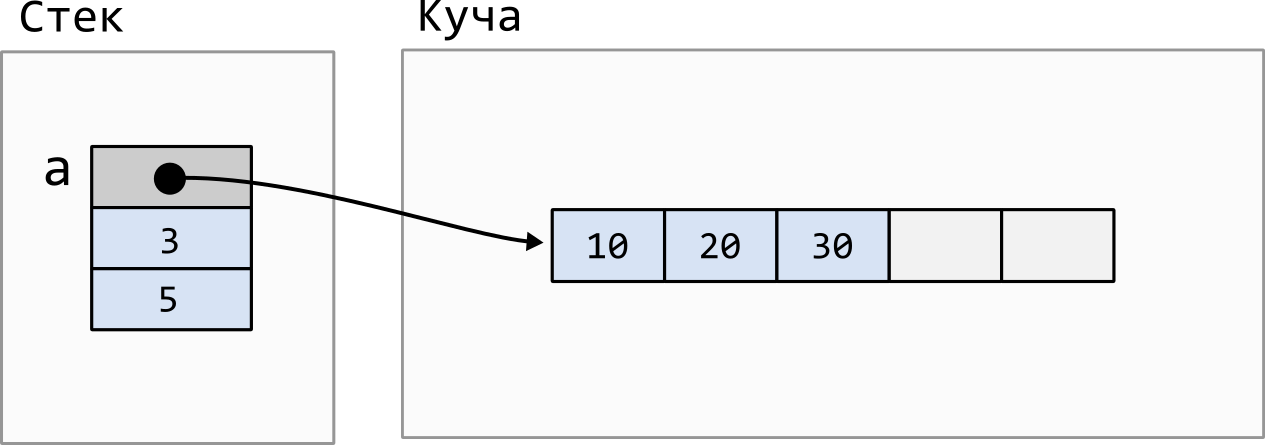
\includegraphics[scale=1]{../images/vector.png}
\end{center}


\subsection*{Методы класса \texttt{std::vector}}
\begin{itemize}
\item Метод \texttt{push\_back} -- добавляет элемент в конец вектора.\\
Метод \texttt{pop\_back} -- удаляет последний элемент вектора.
\begin{lstlisting}
#include <iostream>
#include <vector>

void printVector(const std::vector<int>& v)
{
    for (std::size_t i = 0; i < v.size(); ++i)
        std::cout << v[i] << " ";
    std::cout << std::endl;
}

int main()
{
    std::vector<int> v {10, 20, 30, 40};
    
    v.push_back(50);
    printVector(v);  // Напечатает  10 20 30 40 50
    
    v.pop_back();
    printVector(v);  // Напечатает  10 20 30 40
}
\end{lstlisting}

\item Метод \texttt{front} -- возвращает первый элемент вектора, то же самое, что и \texttt{v[0]}. Метод \texttt{back} -- возвращает последний элемент вектора, то же самое, что и \texttt{v[v.size() - 1]}.
\begin{lstlisting}
#include <iostream>
#include <vector>

int main()
{
    std::vector<int> v {10, 20, 30, 40};
    std::cout << v.front() << " " << v.back() << std::endl;  // Напечатает 10 40
}
\end{lstlisting}

\item Метод \texttt{clear} -- очищает вектор, удаляет все элементы.
\item Метод \texttt{empty} -- возращает \texttt{true}, если вектор пуст и \texttt{false} иначе.
\item Метод \texttt{size} -- возвращает размер вектора.
\item Метод \texttt{capacity} -- возвращает вместимость вектора.
\begin{lstlisting}
#include <iostream>
#include <vector>

int main()
{
    std::vector<int> v {10, 20, 30, 40, 50};
    std::cout << v.size() << " " << v.capacity() << std::endl;  // Напечатает 5 5
    v.push_back(60);
    std::cout << v.size() << " " << v.capacity() << std::endl;  // Напечатает 6 10
}
\end{lstlisting}

\item Метод \texttt{data} -- возвращает указатель на данные в куче. Можно использовать этот метод, если нужно передать вектор в функцию, которая принимает указатель на элемент массива.
\begin{lstlisting}
#include <iostream>
#include <vector>
#include <cstring>

int main()
{
    std::vector<int> v {10, 20, 30, 40, 50};
    
    int a[5];
    std::memcpy(a, v.data(), 5 * sizeof(int));
    
    for (std::size_t i = 0; i < 5; ++i)
        std::cout << a[i] << " ";
    std::cout << std::endl;
}
\end{lstlisting}
\end{itemize}

\subsection*{Операторы, которые можно применять к вектору}
Вектора можно присваивать. Также вектора можно сравнивать. Сравнение происходит в лексикографическом порядке.
\begin{lstlisting}
#include <iostream>
#include <vector>

int main()
{
    std::vector<int> v {10, 20, 30, 40, 50};
    std::vector<int> u;
    
    u = v;
    if (u >= v)
        std::cout << "Yes" << std::endl;
}
\end{lstlisting}


\subsection*{Передача вектора в функции}
Также как и для строки, при передаче вектора в функцию, которая принимает по значению, происходит глубокое копирование вектора, что может быть очень медленно. Поэтому вектор желательно передавать по ссылке. Вектор следует передавать по обычной ссылке, если вектор нужно изменить внутри функции, и по константной ссылке, если в функции вектор меняться не будет.
\begin{lstlisting}
#include <iostream>
#include <vector>
#include <string>
using std::cout, std::endl, std::size_t;

void printVector(const std::vector<std::string>& v)
{
    for (size_t i = 0; i < v.size(); ++i)
        cout << v[i] << " ";
    cout << endl;
}

std::vector<std::string> getAnimals()
{
    std::vector<std::string> result {"Cat", "Dog", "Spider", "Lion", "Snake", "Shark"};
    return result;
}

void eraseLastLetters(std::vector<std::string>& v)
{
    for (size_t i = 0; i < v.size(); ++i)
    {
        if (!v[i].empty())
            v[i].pop_back();
    }
}

std::vector<std::string> getAnimalsByLetter(const std::vector<std::string>& v, char c)
{
    std::vector<std::string> result;
    for (size_t i = 0; i < v.size(); ++i)
    {
        if (v[i].starts_with(c))
            result.push_back(v[i]);
    }
    return result;
}

int main()
{
    std::vector<std::string> a = getAnimals();
    printVector(a);  // Cat Dog Spider Lion Snake Shark
    
    eraseLastLetters(a);
    printVector(a);  // Ca Do Spide Lio Snak Shar
    
    std::vector<std::string> b = getAnimalsByLetter(a, 'S');
    printVector(b);  // Spide Snak Shar
}
\end{lstlisting}






\newpage
\section*{Приведение типов. Оператор \texttt{static\_cast}}

\subsection*{Опасность приведения в стиле C}
Язык C++ унаследовал от языка C приведение типов через круглые скобочки.
Такое приведение через круглые скобочки в C++ называется как \textit{приведение в стиле C} (англ. \textit{C-style cast}).
Однако приведение в стиле C может делать слишком много и оно может быть небезопасно в некоторых ситуациях. Рассмотрим эти ситуации:

\begin{enumerate}
\item \textbf{Приведение типов в стиле C может убирать \texttt{const} у указателей и ссылок}\\
Когда мы передаём объект в функцию, которая принимает по константному указателю, то мы предполагаем, что внутри функции этот объект не изменится. Почти всегда это так, но, в теории, константный указатель внутри функции может быть приведён к обычному указателю с помощью приведения в стиле C.
\begin{lstlisting}
#include <iostream>
using std::cout, std::endl;

void printByAddress(const int* p)
{
    cout << *p << endl;
    
    int* q = (int*)p;
    *q += 10;
}

int main()
{
    int a = 10;
    printByAddress(&a); // Передаём по const int* и думаем, что a внутри не поменяется
    cout << a << endl;  // Напечатает 20
}
\end{lstlisting}

\item \textbf{Приведение типов в стиле C может конвертировать типы указателей без ограничений}\\
Можно, например, конвертировать указатель \texttt{int*} в указатель \texttt{float*}. Если после этого конвертированный указатель будет разыменован, то это приведёт к неопределённому поведению из-за нарушения строгих правил алиасинга.
\begin{lstlisting}
#include <iostream>

int main()
{
    int a = 10;
    int* p = &a;
    
    float* q = (float*)p;
    *q = 1.0;  // UB
}
\end{lstlisting}
Но в редких случаях такое приведение указателей может быть полезно. Во-первых, есть исключения из строгих правил алиасинга, например можно указателем \texttt{char*} указывать на объект типа \texttt{int}. Во-вторых, строгие правила алиасинга можно просто отключить.
\end{enumerate}

Из-за того, что C++ должен быть обратно совместим с языком C, в языке C++ осталось небезопасное приведение через круглые скобочки. Но использование приведение в стиле C считается плохим стилем кода. Его не следует использовать. Вместо этого следует использовать операторы приведения языка C++: \texttt{static\_cast} \texttt{const\_cast}, \texttt{reinterpret\_cast}.


\newpage
\subsection*{Оператор приведения \texttt{const\_cast}}
Оператор приведения \texttt{const\_cast} нужен только для того, чтобы убирать или добавлять \texttt{const} у типов указателей и ссылок. Этот оператор приведения считается небезопасным и его использование запрещено.
\begin{lstlisting}
#include <iostream>
using std::cout, std::endl;

void print(const int& a)
{
    cout << a << endl;
    int& b = const_cast<int&>(a);
    b += 10;
}

int main()
{
    int a = 10;
    print(a);           // Передаём по константной ссылке и думаем, что a внутри не поменяется
    cout << a << endl;  // Напечатает 20
}
\end{lstlisting}

\subsection*{Оператор приведения \texttt{reinterepret\_cast}}
Оператор приведения \texttt{reinterepret\_cast} нужен для того, чтобы конвертировать разные типы указателей и ссылок. Например, он может конвертировать \texttt{int*} в \texttt{float*}. Этот оператор приведения считается небезопасным, так как можно легко нарушить правила строгого алиасинга, но иногда его необходимо использовать.
\begin{lstlisting}
#include <iostream>

int main()
{
    int a = 10;
    int* p = &a;
    
    char* qc = reinterpret_cast<char*>(p);
    *qc = 0xaa;  // OK, так как char* является исключением из строгих правил алиасинга
    
    float* qf = reinterpret_cast<float*>(p);
    *qf = 1.0;   // UB, нарушены строгие правил алиасинга
}
\end{lstlisting}

\subsection*{Оператор приведения \texttt{static\_cast}}
Оператор приведения \texttt{static\_cast} нужен для всего остального. Он считается относительно безопасным и его следует использовать всегда, когда нужно сделать приведение типов. Остальные типы приведений следует использовать только если \texttt{static\_cast} не подходит.
\begin{lstlisting}
#include <iostream>

int main()
{
    int a = 10;
    float b = static_cast<float>(a);
}
\end{lstlisting}

\newpage
\section*{Другие различия между C и C++}
\subsection*{В C++ нет неявного приведения из \texttt{void*} в указатель другого типа}
В обоих языках нет неявного приведения одного типа указателя к другому в общем случае:
\begin{lstlisting}
int main()
{
    int a = 10;
    int* p = &a;
    float* q = p;  // Ошибка в обоих языках
}
\end{lstlisting}
Но есть неявное приведение в некоторых ситуациях:

\begin{itemize}
\item Из обычного указателя в константный указатель того же типа:
\begin{lstlisting}
int main()
{
    int a = 10;
    int* p = &a;
    const int* q = p;  // OK в обоих языках
}
\end{lstlisting}

\item Если один тип является \texttt{typedef}-ом другого:
\begin{lstlisting}
#include <stdio.h>
int main()
{
    unsigned long long a = 10;
    unsigned long long* p = &a;
    size_t* q = p;  // OK в обоих языках, на 64-х битных системах
}
\end{lstlisting}

\item Из числового литерала, равного нулю:
\begin{lstlisting}
int main()
{
    int* p = 0;  // OK в обоих языках
}
\end{lstlisting}

\item Из типа указателя к типу \texttt{void*}:
\begin{lstlisting}
int main()
{
    int a = 10;
    int* p = &a;
    void* q = p;  // OK в обоих языках
}
\end{lstlisting}


\item Из указателя типа \texttt{void*} к типу \texttt{int*}:
\begin{lstlisting}
int main()
{
    int a = 10;
    void* p = &a;
    int* q = p;  // OK в C, Ошибка в C++
}
\end{lstlisting}
В языке C++ запрещён такое неявное приведение для безопасности. Такое неявное приведение может привести к ошибкам.

\end{itemize}


\subsection*{В C++ нужно использовать константу \texttt{nullptr} для нулевых указателей}
В языке C для нулевого указателя использовуется константа \texttt{NULL}. В языке C++ её тоже можно использовать, но нежелательно, вместо этого лучше использовать новую константу \texttt{nullptr}.

Причина этого в том, что \texttt{NULL} является просто макро-константой определёной в стандартной библиотеке, например, так:
\begin{lstlisting}
#define NULL 0
\end{lstlisting}
В разных компиляторах это определение может быть разным, то есть \texttt{NULL} может быть разного типа.
В языке C++ это может привести к различным проблемам:
\begin{lstlisting}
#include <iostream>
void func(int a)  {std::cout << "Int"     << std::endl;}
void func(int* p) {std::cout << "Pointer" << std::endl;}

int main()
{
    int* p = NULL;
    func(p);        // Напечатает Pointer
    func(NULL);     // Ошибка, в зависимости от компилятора может выбрать первую перегрузку 
                    // или привести к ошибке компиляции
}
\end{lstlisting}
В языке C++ сделали новый указатель \texttt{nullptr}, который имеет уникальный тип \texttt{nullptr\_t}. При этом \texttt{nullptr} может неявно приводится к любому типу указателя. Это избавляет от проблемы, когда компилятор мог спутать \texttt{NULL} с нулём.
\begin{lstlisting}
#include <iostream>
void func(int a)  {std::cout << "Int"     << std::endl;}
void func(int* p) {std::cout << "Pointer" << std::endl;}

int main()
{
    int* q = nullptr;
    func(q);        // Напечатает Pointer
    func(nullptr);  // Напечатает Pointer
}
\end{lstlisting}

\subsection*{Параметры функций со значением по умолчанию}
Язык C++ поддерживает параметры функций со значением по умолчанию. Для это нужно просто задать значения по умолчанию в объявлении функции:
\begin{lstlisting}
#include <iostream>
void func(int a, int b = 10, std::string prefix = "Hello: ")
{
    std::cout << prefix;
    std::cout << a + b << std::endl;
}

int main()
{
    func(10, 20, "Hi: ");  // Напечатает Hi: 30
    func(10, 20);          // Напечатает Hello: 30
    func(10);              // Напечатает Hello: 20
}
\end{lstlisting}
В целом, это неудачное нововведение C++. Использование таких функций является плохим стилем кода. 


\subsection*{Форматированный вывод с использованием \texttt{std::cout}}

\subsubsection*{Печать в шестнадцатеричной системе счисления}
\begin{lstlisting}
#include <iostream>
using std::cout, std::endl;

int main()
{
    int a = 200;
  
    cout << std::hex;   // Переключить печать в 16-ричную систему
    cout << a << endl;  // Напечатает  c8
    cout << a << endl;  // Напечатает  c8
    cout << std::dec;   // Переключить печать в 10-ичную систему
    cout << a << endl;  // Напечатает  200
}
\end{lstlisting}


\subsubsection*{Печать чисел с плавающей точкой с заданием количества знаков после точки}
Используем \texttt{std::setprecision} из библиотеки \texttt{iomanip}.
\begin{lstlisting}
#include <iostream>
#include <iomanip>
#include <cmath>
using std::cout, std::endl;

int main()
{
    double x = std::sqrt(2);
    cout << x << endl;  // Напечатает  1.41421
    
    cout << std::setprecision(20);
    cout << x << endl;  // Напечатает  1.4142135623730951455
}
\end{lstlisting}

\subsubsection*{Печать чисел с фиксированной шириной и с замощением другими символами}
Используем \texttt{std::setw} и \texttt{std::setfill} из библиотеки \texttt{iomanip}.
\begin{lstlisting}
#include <iostream>
#include <iomanip>
using std::cout, std::endl;

int main()
{
    int a = 123;
    
    // Следующая строка напечатает | {} 123|
    cout << "|" << std::setw(5) <<   a << "|" << endl;
    
    // Следующая строка напечатает |00123|
    cout << "|" << std::setw(5) <<  std::setfill('0') << a << "|" <<  endl;
}
\end{lstlisting}
\end{document}
